\documentclass[a4paper, 12pt,oneside,reqno]{amsart}
\usepackage[utf8x]{inputenc}
\usepackage[T1]{fontenc}
\usepackage{tikz}
\usetikzlibrary{arrows,shapes,snakes,automata,backgrounds,petri,through,positioning}
\usetikzlibrary{intersections}
\usepackage{tikz-cd}
\usepackage{amssymb,amscd,amsthm,amsmath}
\usepackage{amsmath}
\usepackage{amssymb}
\usepackage[colorinlistoftodos]{todonotes}
\usepackage[colorlinks=true, allcolors=blue]{hyperref}

\begin{document}

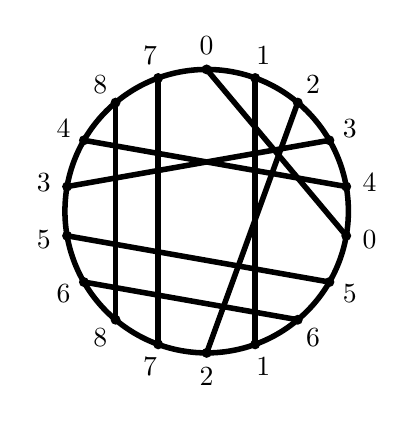
\begin{tikzpicture}[scale=0.6]
        \draw[line width =2] (0,0) circle (3);
     
     {\foreach \angle/ \label in
   { 90/0, 110/7, 130/8, 150/4, 170/3, 190/5, 210/6, 230/8, 250/7, 
     270/2, 290/1, 310/6, 330/5, 350/0, 10/4, 30/3, 50/2, 70/1 }
   {
    \fill(\angle:3.5) node{$\label$};
    \fill(\angle:3) circle (3pt) ;
    }
}

  \draw[line width = 2] (90:3) -- (350:3);
  \draw[line width = 2] (70:3) -- (290:3);
  \draw[line width = 2] (50:3) -- (270:3);
  \draw[line width = 2] (30:3) -- (170:3);
  \draw[line width = 2] (10:3) -- (150:3);
  \draw[line width = 2] (330:3) -- (190:3);
  \draw[line width = 2] (310:3) -- (210:3);
  \draw[line width = 2] (250:3) -- (110:3);
  \draw[line width = 2] (230:3) -- (130:3);

  \end{tikzpicture}

\end{document}